\documentclass[pre,amsmath,amssymb, twocolumn, showpacs]{revtex4-1}
%showpacs, twocolumn
\usepackage{dcolumn}
\usepackage{bm}
\usepackage{graphicx}
\usepackage{hyperref}
\usepackage{mathptmx}
\usepackage{subfigure}
\usepackage[utf8]{inputenc}
\usepackage{bbold}
\usepackage{color}
\newcommand{\david}[1]{{\color{red} #1}}
\newcommand{\ata}[1]{{\color{blue} #1}}
\newcommand{\pp}{p_{al}}
\makeatletter

\begin{document}

\title{Efficient algorithm for the periodic Lorentz gas in 2 and 3 dimensions}
\author{Atahualpa S.~Kraemer}
\email{ata.kraemer@gmail.com}
\affiliation{Institut für Theoretische Physik II - Soft Matter
Heinrich-Heine-Universität Düsseldorf
Building 25.32
Room O2.56
Universitätsstrasse 1
D-40225 Düsseldorf, Germany}

\author{Nikolay Kryukov}
\email{kryukov@ciencias.unam.mx}

\author{David P.~Sanders}
\email{dpsanders@ciencias.unam.mx}
\affiliation{Departamento de F\'isica, Facultad de Ciencias, Universidad Nacional
Aut\'onoma de M\'exico,
Ciudad Universitaria, M\'exico D.F.\ 04510, Mexico
}

\date{\today}
\begin{abstract}

We present an efficient algorithm to calculate collisions for a periodic Lorentz gas in two and three dimensions. The 2D algorithm uses continued fractions to obtain the exact disc with which a particle will collide at each step, instead of using periodic boundary conditions. The 3D version uses the 2D algorithm, but obtains these coordinates only with a probability $\pp$ which depends on the size of the obstacles as $\pp \sim 1-0.5 r^3$. We study the efficiency of the algorithm and apply it to calculate free path distributions. The algorithm can be generalized to higher dimensions. 
\end{abstract}

\maketitle

\section{Introduction}



Lorentz gases are simple physical systems that present deterministic chaos \cite{cvitanovic1992investigation}, and are a popular model in statistical mechanics and nonlinear dynamics. This model consists of point particles that move freely until they encounter obstacles, often spheres, where they undergo elastic collisions. 
%When these obstacles are arranged periodically at the vertices of a grid (``periodic Lorentz gas''), the model is equivalent to a Sinai billiard \cite{bunimovich1981statistical}.

These systems can have different configuration of the obstacles, e.g., random lattices \cite{latz1997lyapunov,dellago1997lyapunov, van1998chaotic} or quasiperiodic systems \cite{kraemer2013embedding,wennberg2012free}. However, because of its simplicity, the periodic case has been widely studied (see e.g. \cite{bunimovich1981statistical,bleher1992statistical, chernov1994statistical, gilbert2011diffusive}); in this case, the model is equivalent to a Sinai billiard  \cite{bunimovich1981statistical}. There are still many open questions in this area\cite{gilbert2009persistence,marklof2011periodic,nandori2012tail, dettmann2012new}. Many of the results obtained theoretically for these gases are in the limit where obstacles are very small, i.e., the so-called Boltzmann--Grad limit \cite{caglioti2003distribution, golse2012recent,boca2007distribution,golse2006periodic,caglioti2008boltzmann,caglioti2010boltzmann, golse2000distribution,marklof2008kinetic, bourgain1998distribution}. 

The standard simulation method for periodic Lorentz gases is to reduce to a single cell, with periodic boundary conditions, and, in the simplest case, an obstacle in the centre of the cell\cite{sanders2005fine, sanders2008normal}. However, this implies that the program must check each time that the particle crosses a border whether it will collide with the obstacle in the cell, or if it will move to the next cell. That implies solving at least two linear equations and one quadratic, then checking if the solution of the quadratic equation is real and finally taking the maximum value of the two or three results. If the obstacle is big enough, it is quite probable that the particle will collide each time it crosses the boundary. However, in the Boltzmann--Grad limit, this situation does not happen very often, and then much time is lost in unnecessary checks.

A suitable situation would be a formula to find the coordinates of the next obstacle giving the position and velocity of the particle. As we will see in section \ref{algorithm} this is indeed the first solution of the Diophantine inequality:

\begin{equation}
|\alpha q+b-p|\leq  \frac{v^2}{v_x} r
\end{equation}

where $r$ is the radius of the obstacles, $q$ and $p$ are integer variables, and $\alpha$ and $b$ are two real numbers related to the position $\vec{x}$ and velocity $\vec{v}$ of the particle. But this inequality is closely related to the best rational approximant to an irrational number for the case $b=0$ and the solutions can be obtained by the continued fraction algorithm. 

An algorithm for this, using continued fractions, was previously developed; see \cite{zacherl1986power}. However, it was never published. Nevertheless,  continued fractions have often been used to provide information about the free path distribution of the periodic Lorentz gas in the Boltzmann--Grad limit \cite{caglioti2003distribution, golse2012recent,boca2007distribution,golse2006periodic,caglioti2008boltzmann, caglioti2010boltzmann, golse2000distribution, bleher1992statistical,chernov1994statistical}, and, relatively recently, Golse has developed an algorithm to code particles trajectories by using the continued fraction algorithm and the 3-length theorem \cite{golse2012recent}. 

However, this algorithm works a priori only if the particle leaves the surface of a disk. This restriction prevents the algorithm from being used in other geometries, such as quasiperiodic arrays, two incommensurate overlapping arrays of square lattices, or with different shapes of obstacles; such systems may produce a number of surprising effects \cite{marklof2014power}.  On the other hand, due to the construction of the algorithm, using the 3-length theorem and continued fraction algorithm, it is not possible to use it in higher dimensions, which ``is a notoriously more difficult problem'' according to Golse.

\section{2D algorithm}
\label{algorithm}

In this section, we present the 2D algorithm.
Its goal is to calculate efficiently where the first collision of a particle will occur in a square lattice. Without loss of generality, we will use the lattice formed by the integer coordinates in the 2D plane. Then, we want to calculate the minimal time $t^{\ast}>0$, such that a collision occurs with some disc with centre $\vec{c}=(q,p)$, with $q$ and $p$ integers. The condition is then 
$\| \vec{c}-(\vec{x_0}+\vec{v_0} \, t^{\ast}) \| = r$, where $r$ is the radius of the obstacle, and $\vec{x_0}$ and $\vec{v_0}$ are the initial position and velocity of the particle. In this case, the collision takes place at the point $\vec{x_0}+\vec{v_0} t^{\ast}$.

\subsection{Collision with disc}
The classical algorithm finds the intersection between a line corresponding to the trajectory of 
the particle and a circle. A first improvement follows from observing that instead we may look for the intersection with another line instead. We denote by $(v_{1}, v_{2})$ the components of the particle's velocity. Without loss of generality we take the speed to be 1, and $v_1>0$ and $v_2>0$ in the following; we can always rotate or reflect the system such that these conditions are satisfied, due to its symmetry.

We write the equation of the particle's trajectory as $y=\alpha x+b$ and look for its intersection with the vertical line $x=q$. As shown in figure~\ref{fig:circle}, if $|\alpha q+b-p| = |b| < \delta := r/v_1$, then a collision will take place. Due to the periodic boundary conditions, we can always put $0 < b < 1$, so we only need to solve $b<\delta$. This gives us a tool to calculate with which obstacle the particle will collide. 

Indeed, we do not need to apply periodic boundary conditions at every step, we only need to check 
\begin{equation}
|\{ \alpha  q_n \}+b -1|< \delta, 
\label{eq:master}
\end{equation}
where $\{ \cdot \}$ denotes the fractional part, and $q_n=q_{n-1}+1$, where $q_1$ is the $x$-coordinate of the closest obstacle to the particle at $t=0$. Then, the first $q_n$ that satisfies this inequality will be $q$. To calculate $p$, we can note that always $p=\lfloor \alpha q +b\rfloor$ or $p=\lfloor \alpha q +b\rfloor+1$

\begin{figure}
\centering
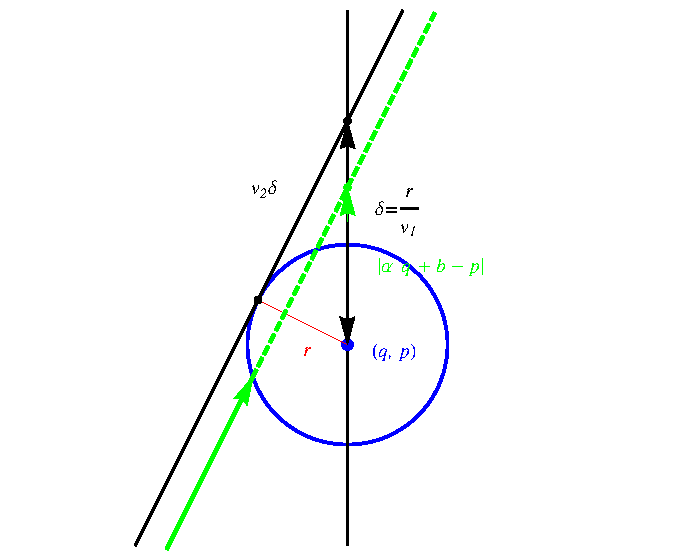
\includegraphics [width=240pt]{fig01.pdf}
\caption{Relation between the intersection of a line and a circle with integer coordinates and the intersection of the line $x = q$. }
\label{fig:circle}
\end{figure}


Now, to simplify even more the algorithm, consider the integer coordinates $(q_n, p_n)$ such that
\begin{equation}
|\alpha q_n -p_n + b|< \delta,
\label{eq:1}
\end{equation}
and for any pair of numbers $(i,j)$ such that $i<q_n$, then $|\alpha i -j+ b|> \delta$,  $q=q_n$, and $p=p_n$. 
 
But $|\alpha q_i - p_i + b|$ are the distances between the integer coordinates $(q_i, p_i)$ and the point $( q_i ,\alpha q_i + b)$. Thus, we would like a sequence such that  
\begin{equation}
|\alpha q_i - p_i + b|<|\alpha q_{i-1} - p_{i-1} + b|
\label{eq:iteration}
\end{equation}
for every $i>1 \in   \mathbb{N}$. Also, the first pair of integer coordinates $q_0$ and $p_0$ should be $(0, 0)$ or $(0, 1)$, minimizing $|\alpha q_0 - p_0 + b|$, that is:

\begin{equation}
|\alpha q_1 -p_1 + b|< f(b) = \begin{cases} b &\mbox{if } b < 1/2 \\ 
1-b & \mbox{if } b > 1/2 \end{cases} .
\label{eq:prima}
\end{equation}

Note that $p_n= \lfloor \alpha q_n +b  \rfloor= \begin{cases} \lfloor \alpha q_n  \rfloor  &\mbox{if } b+\alpha q_n-\lfloor \alpha q_n  \rfloor < 1 \\ 
 \lfloor \alpha q_n  \rfloor+1  &\mbox{if } b+\alpha q_n-\lfloor \alpha q_n  \rfloor > 1 \end{cases}$ if $b<1/2$ or $p_n= \lfloor \alpha q_n +b  \rfloor+1= \begin{cases} \lfloor \alpha q_n  \rfloor+1  &\mbox{if } b+\alpha q_n-\lfloor \alpha q_n  \rfloor < 1 \\ 
 \lfloor \alpha q_n  \rfloor+2  &\mbox{if } b+\alpha q_n-\lfloor \alpha q_n  \rfloor > 1 \end{cases}$ if $b>1/2$. Substituting the four cases form here in the two cases of equation \ref{eq:prima}, we obtain that indeed $p_1= \lfloor \alpha q_1  \rfloor+1$, and then,  iterating  inequality \ref{eq:iteration} we obtain 
 %
\begin{equation}
 p_n= \lfloor \alpha q_n  \rfloor+1.
\label{eq:hn}
\end{equation}
 
Mixing the inequality \eqref{eq:1} and equation \eqref{eq:hn}, we obtain again equation \eqref{eq:master}. 

Thus, we have reduced the solution from two linear equations and one quadratic to one linear equation. Furthermore, now we do not check in every periodic cell, because if $\alpha >1$, for every $q_n$ we advance $\alpha$ cells. And we do not need to apply periodic boundary conditions until we reach the obstacle. 

\subsection{The Diophantine inequality: $|\alpha p - q|\leq \epsilon$}

Now, a better algorithm should find a way to find the set of $q_i$, such that inequality \eqref{eq:iteration} holds for every $i$, and there is no integer $q$  such that $q_i<q<q_{i-1}$ for some $i$ and
$|\{ \alpha  q_i \}+b -1|<|\{ \alpha  q \}+b -1| <|\{ \alpha  q_{i-1} \}+b -1|$. 

In order to do this, we can use the continued fraction algorithm to obtain solutions to the inequality $|\alpha q - p|\leq \epsilon$. This algorithm already gives a sequence of $(q_n,p_n)$ such that $|\alpha q_i - p_i|<|\alpha q_{i-1} - p_{i-1}|$ if $q_{i-1} <q_i$. So, if we turn our inequality \eqref{eq:prima} into this other inequality, we will find our algorithm just by using the continued fraction algorithm.
Indeed, using equation \ref{eq:hn} and the inequality \ref{eq:prima}, we obtain $|\{ \alpha  q_1 \} -1|< \begin{cases} 2b &\mbox{if } b < 1/2 \\  2(1-b) & \mbox{if } b > 1/2 \end{cases} $, which is almost the continued fraction inequality, except that $p$ is always equal to $\lfloor \alpha q  \rfloor+1$. 

\begin{equation}
|\alpha  q-p|< \begin{cases} 2b &\mbox{if } b < 1/2 \\  2(1-b) & \mbox{if } b > 1/2 \end{cases}
\label{eq:master2}
\end{equation}

Then, we can apply the continued fraction algorithm to obtain $p$ and $q$ of inequality \eqref{eq:master2}. If $\lfloor \alpha q  \rfloor+1$, then, we have found $(q_1,p_1)$, otherwise not, but we know that $p_1\geq p$, and $q_1 \geq q$, so we can just use $(q, p)$ even if they do not satisfy inequality \ref{eq:iteration}, then calculate the sequence $b_i$ as $b_0=b$, $b_i=\{\alpha q_i+b\}$. If $b_n<\delta$ the algorithm stops, and the collision will take place with the obstacle centred at the coordinates $(q_n,p_n)$. 

\subsection{Explicit algorithm}

Now we have all the necessary tools to implement the complete algorithm step by step. The Julia language \cite{julialang} is used; the source code is available at ???

The function \texttt{frac($\alpha, \epsilon$)} calculates the first integers $(q,p)$ such that 
$|\alpha q-p|<\epsilon$ by using the continued fraction algorithm; see the appendix. This is used to calculate which disc is hit by the following function

Now, define the function \texttt{eff(m, b, r)} as follows: 
\begin{verbatim}
function eff(m, b, r)
	kn = 0
    b1 = b
    epsilon = r*sqrt(m*m+1) 
    if(b < epsilon || 1 - b < epsilon)
        if b < BigFloat("0.5")
			(q, p) = frac(m, 2.*b)
		else
			(q, p) = frac(m, 2.*(1. - b))
		end
		b = mod(m*q + b, 1)
		kn += q
    end  
	while b > epsilon && 1 - b > epsilon
		if b < BigFloat("0.5")
			(q, p) = frac(m, 2.*b)
		else
			(q, p) = frac(m, 2.*(1. - b))
		end
		b = mod(m*q + b, 1)
		kn += q
	end
	q = kn
    p = int(m*q+b1)
    return [q, p]
end
\end{verbatim}

This function applies the continued fraction algorithm along with the inequality \ref{eq:master2} until the distance in the y-direction between the line and the integer coordinates $(q, p)$ is less than $\epsilon$. 

Then, the algorithm to localize the first obstacle, with which a particle with velocity $\vec{v}$ and position $\vec{x}$ will collide, is as follows (in pseudocode): 

\begin{verbatim}
if (v is in quadrant I) then     
   (q,p)=efficient_algorithm(m, b, delta)
   p=int(m*q)+1
else if (v is in quadrant II) then
   m=-m                               
   % reflect the system with 
   %respect to y-axis 
   (q,p)=efficient_algorithm(m, b, delta)
   p=int(m*q)+1
   m=-m                                
   % reflect the system with 
   %respect to y-axis
   q=-q                                
   % reflect the system with 
   %respect to y-axis
else if (v is in quadrant III) then
   b=1-b                              
   % reflect the system with 
   %respect to the origin
   (q,p)=efficient_algorithm(m, b, delta)
   b=1-b                              
   % reflect the system with 
   %respect to the origin
   p=-(int(m*q)+1)                               
   % reflect the system with 
   %respect to the origin
   q=-q                               
   % reflect the system with 
   %respect to the origin
else if (v is in quadrant IV) then
   b=1-b                              
   % reflect the system with 
   %respect to the x-axis
   m=-m                               
   % reflect the system with 
   %respect to the x-axis
   (q,p)=efficient_algorithm(m, b, delta)             
   b=1-b                              
   % reflect the system with 
   %respect to the x-axis
   m=-m                               
   % reflect the system with 
   %respect to the x-axis
   p=-(int(m*q)+1)                               
   % reflect the system with 
   %respect to the x-axis
endif
\end{verbatim}

Using the technique mentioned above, which, for the initial position $(0, b), 0 < b < 1$ and for any initial velocity returns the integer coordinates of the obstacle of the first collision, we make the function \texttt{Lorentz(x, v, r)} that calculates the first collision of the particle in the 2D plane. In order to calculate the exact collision point and the velocity after the collision, we need to use the classical collision functions \texttt{collision} and \texttt{velo\_col}.

\section{3D algorithm}

In this section, we present an efficient algorithm for calculating the next collision with a sphere in 3D on a simple cubic lattice. The algorithm works by projecting to 2D planes and using the 2D algorithm in each plane, as follows.

Suppose we project a particle trajectory in a 3D lattice onto one of the $x$--$y$, $x$--$z$ or 
$y$--$z$ planes. We will obtain a periodic square lattice with a 2D trajectory, but with a speed that is, in general, not $1$. 
Thus, we can apply the 2D algorithm for each of the 3 projections, and obtain the coordinates of 3 obstacles in the 3 projected planes where the first collision occurs.  

We now check whether the obstacle coordinates in these projections correspond to the same 3D obstacle. If so, then we check if the particle really does collide with this obstacle by using the standard method; if it does, then we return the coordinates of the obstacle, and if not, we move the particle to the next cell and continue applying the algorithm. If the projections do not correspond to the same 3D obstacle, we move the particle to the cell containing the obstacle that is furthest away, and continue.

%Some times the particle in the projected planes is inside of an obstacle. 
%If this happens, then we considered that the collision occurs with that obstacle. 

Using the 2D continued fraction algorithm in one of the planes $xy$, $xz$ and $yz$ is equivalent to calculating the first collision with a cylinder orthogonal 
to that plane. Joining those coordinates together is equivalent to calculating a collision with the intersection of the three orthogonal cylinders with the same radius. 

Figure~\ref{fig:collision} shows the intersection of the 3 cylinders, together with a sphere of the same radius. The sphere is contained inside the intersection of the cylinders; the 
 regions outside the sphere correspond to places where the 3D algorithm does not find the correct next collision, even when the three 2D obstacles coincide.
 
\begin{figure}
\centering
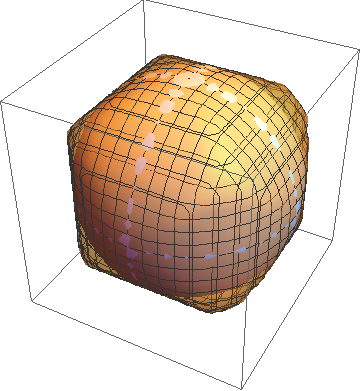
\includegraphics [width=240pt]{./region.png}
\caption{A sphere of radius $r$ embedded into the intersection of 3 orthogonal cylinders of the same radius. The volume where there is no sphere, but there is the intersection of the 3 cylinders, is the place where trajectories of particles can be considered as having collisions, when really they do not use the proposed algorithm in the 3D case.}
\label{fig:collision}
\end{figure}

 
 The probability that this occurs is the volume of the intersection of the cylinders minus the volume of the sphere:
%As Figure \ref{fig:collision} suggests, the difference $\pp$ between the real obstacle and the intersection of the cylinders is not large. 
% In other words, the probability $\pp$ that the 3D algorithm will find the collision in the first coincidence is: 
%
\begin{equation}
\pp= 1-(16-\sqrt{128}-\frac{4}{3} \pi) r^3 \sim 1-0.5 r^3.
\end{equation}
This is very small for small obstacles; for example, obstacles of radius $r=0.01$ give a probability $\pp \sim 0.999995$.

\section{Numerical measurements}

In order to test how efficient our algorithm is, we measured the average time of the execution of the function finding the first collision starting from the initial point around the origin,
 depending on the radius of the obstacle, for both the classical and efficient algorithms.

\begin{figure}
\centering
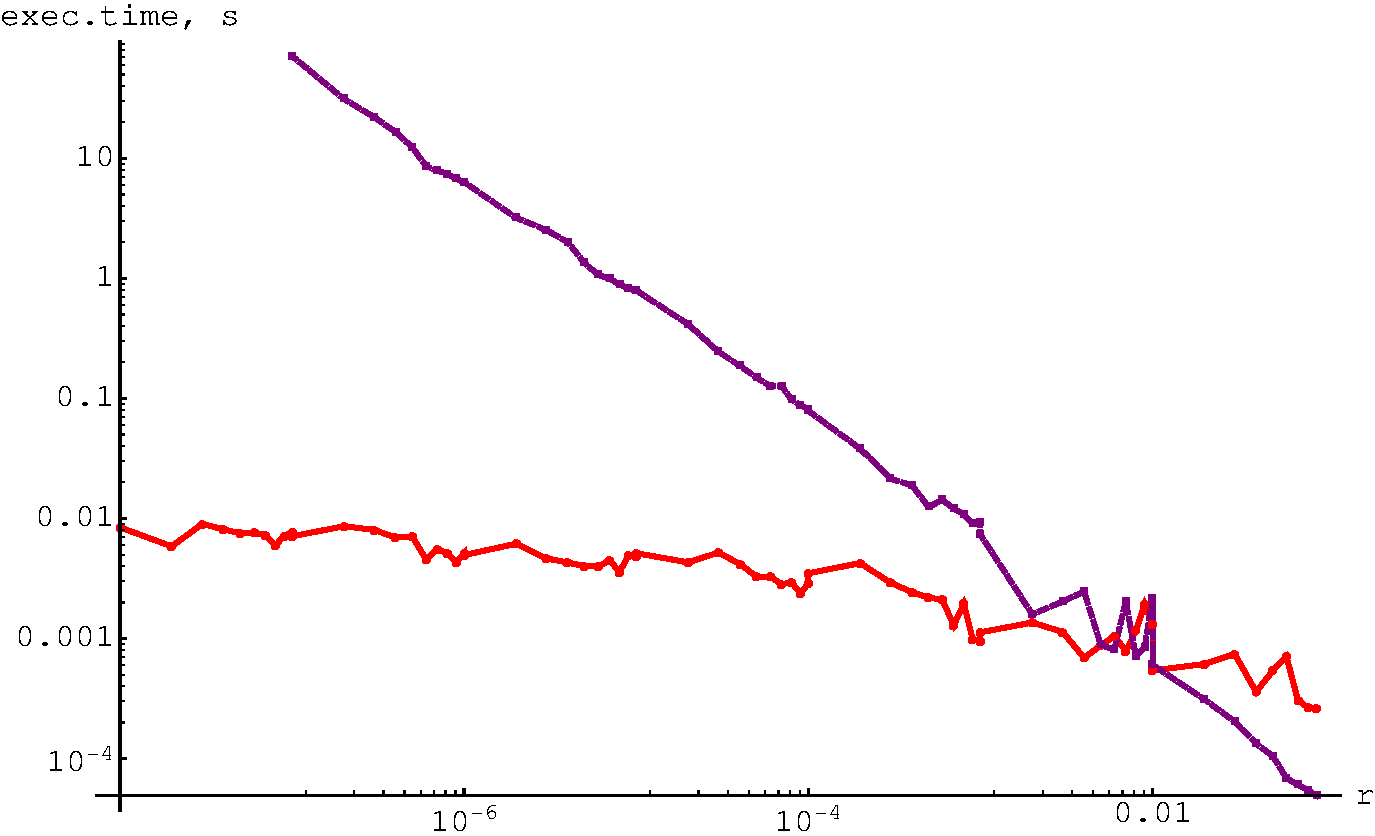
\includegraphics [width=260pt]{fig03.pdf}
\caption{Average execution time of finding the first collision in 2D Lorentz gas, for the classical (dotted curve) and efficient (solid curve) algorithms.}
\label{fig:fig05}
\end{figure}

\begin{figure}
\centering
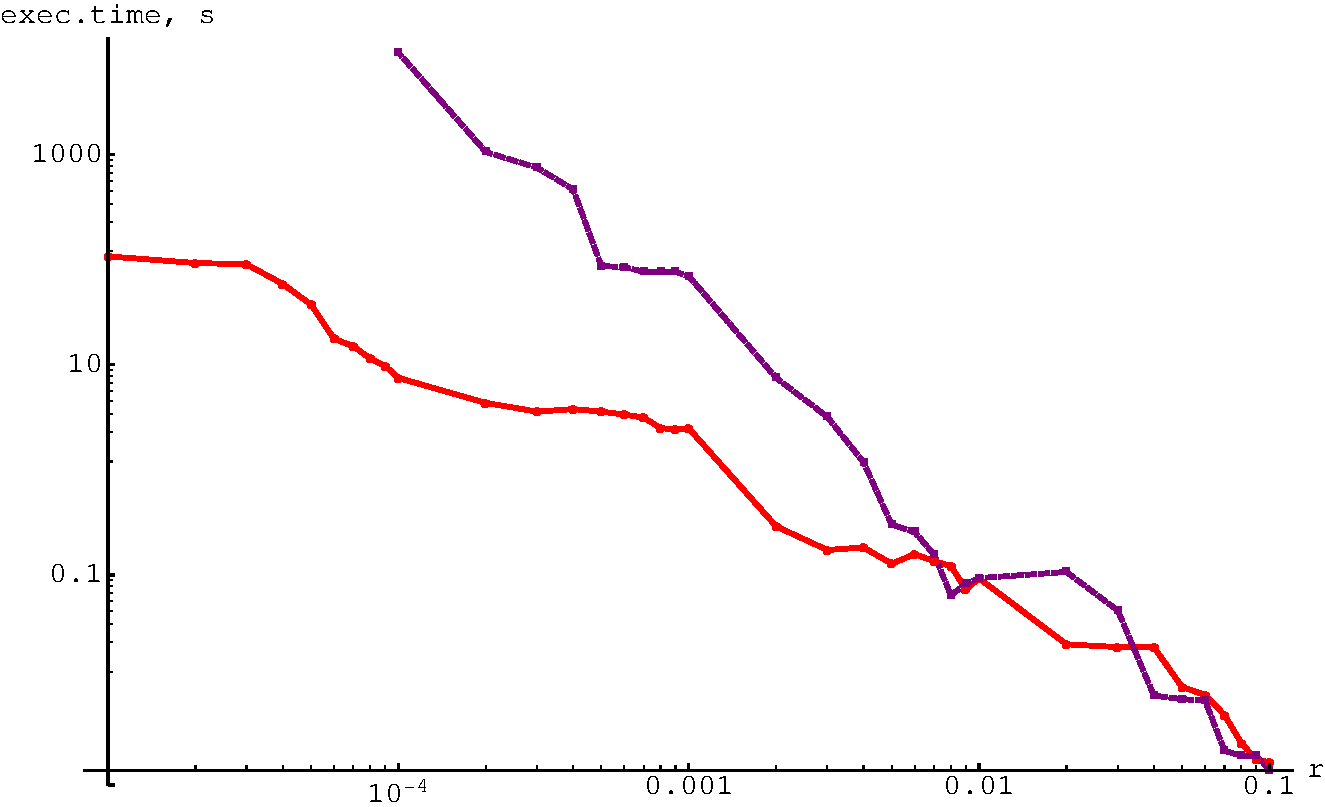
\includegraphics [width=260pt]{fig04.pdf}
\caption{Average execution time of finding the first collision in 3D Lorentz gas, for the classical (dotted curve) and efficient (solid curve) algorithms.}
\label{fig:fig06}
\end{figure}

Figures \ref{fig:fig05} and \ref{fig:fig06} show the results for the 2D and 3D algorithms. As we can see, the new algorithm is significantly more efficient for $r < 0.01$.

Similarly, we calculated the execution time per cell depending on the radius of the obstacle, for both 2D and 3D efficient algorithm comparing it to classical. Classical algorithms use periodic boundary conditions, so the execution time per cell is about the same, regardless of the radius of the obstacle. 
For small radii, we can observe the efficiency of this algorithm.

\begin{figure}
\centering
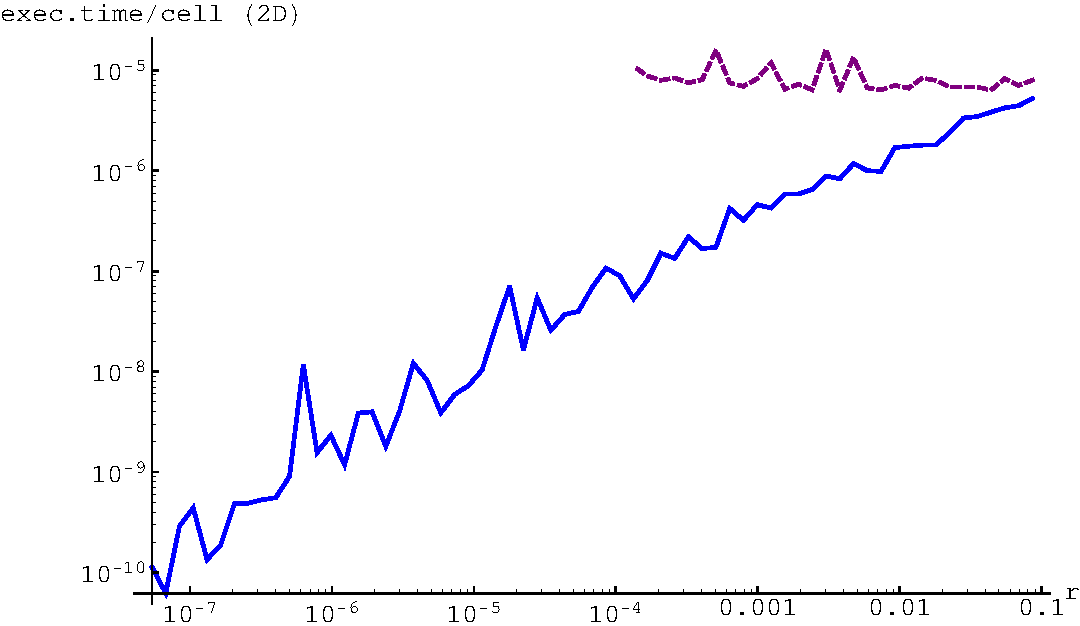
\includegraphics [width=260pt]{exectimepercell-2D.pdf}
\caption{Mean execution time per cell of finding the first collision in 2D Lorentz gas, for the classical (dashed curve) and efficient (solid curve) algorithms.}
\label{fig:exectimepercell2D}
\end{figure}

\begin{figure}
\centering
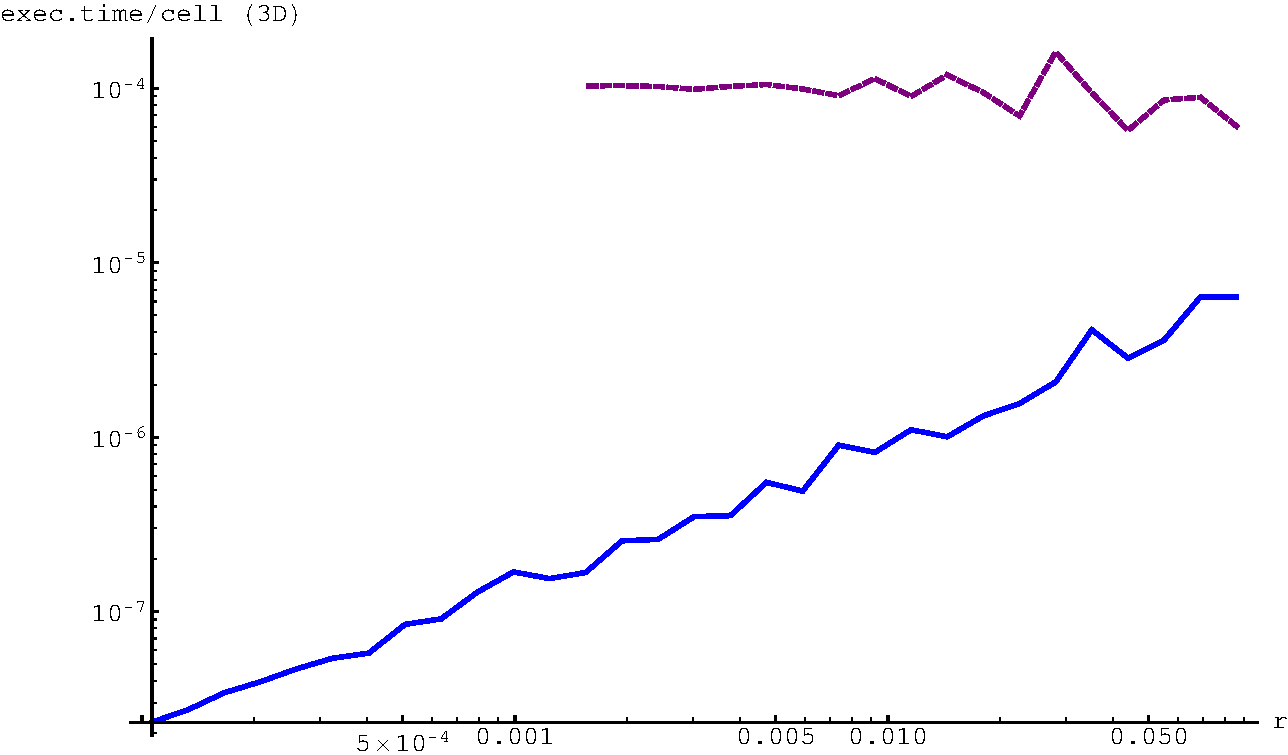
\includegraphics [width=260pt]{exectimepercell-3D.pdf}
\caption{Mean execution time per cell of finding the first collision in 3D Lorentz gas, for the classical (dashed curve) and efficient (solid curve) algorithms.}
\label{fig:exectimepercell3D}
\end{figure}

\subsection{Free flight distribution}
As an example application of our algorithm, we have measured the distribution of free flight lengths for the first collision for certain systems studied by Marklof and Str\"ombergsson \cite{marklof2014power}. They proved the asymptotic decay of the free flight probability density incommensurable, overlapping periodic Lorentz gases in the Boltzmann--Grad limit. 

Figure~ shows our numerical results for this distribution in the case of two and three overlapping lattices, compared to the rigorous result; the distributions obtained numerically do indeed follow the power laws predicted. The minimum time for each lattice is calculated separately, and the minimum of those results is then taken.

\begin{figure}
\centering
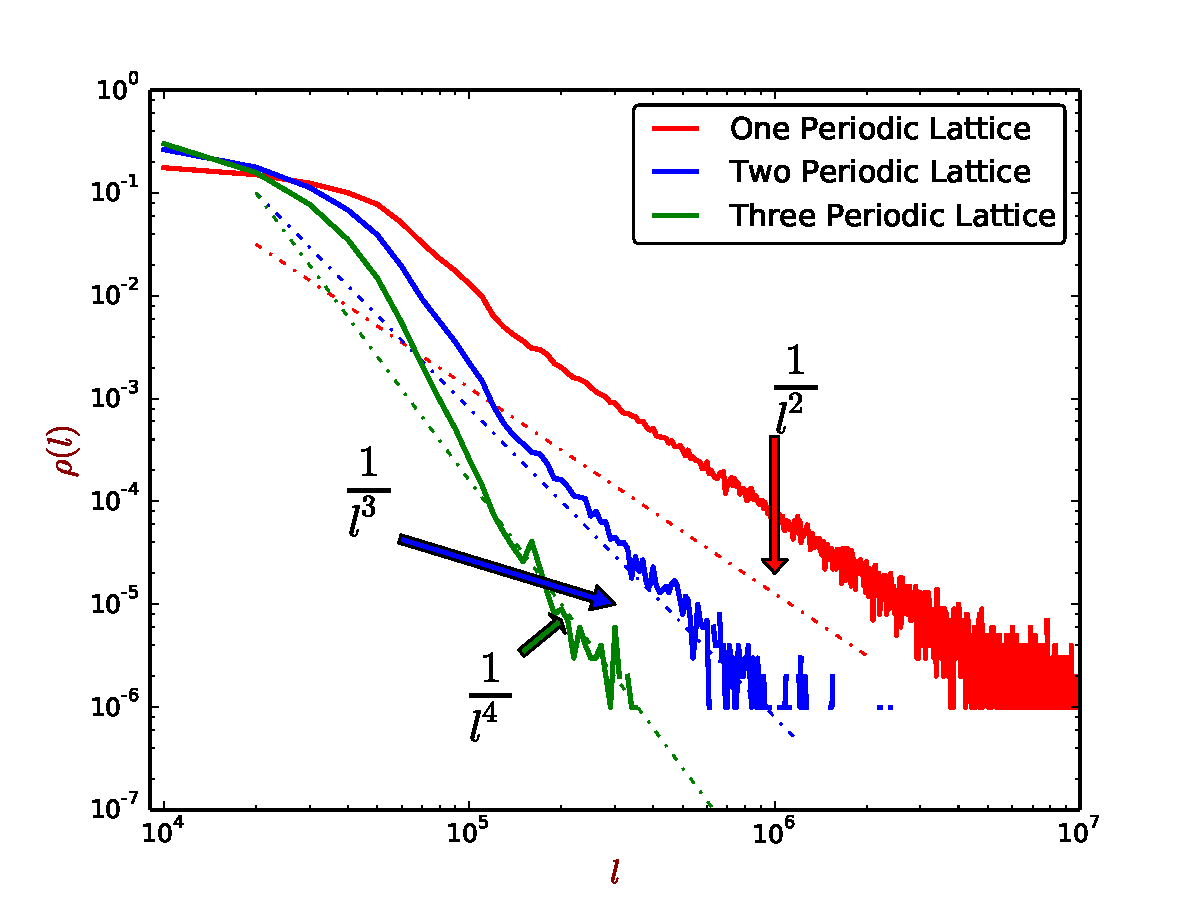
\includegraphics [width=260pt]{Free-Fligth-Rot.pdf}
\caption{Probability density of free flight length for 2 and 3 incommensurable, overlapping periodic Lorentz gases. The results for a single lattice are shown for comparison.}
\label{fig:mark}
\end{figure}

\section{Conclusions}  

We have presented efficient algorithms to simulate periodic Lorentz gases in 2 and 3 dimensions when the obstacles are small and have compared the efficiency of these algorithms with the standard ones, showing that the relative efficiency indeed increases very fast in 2D and fast in 3D.

The 3D algorithm can readily be generalized to higher dimensions. This work is in progress.
We expect that these algorithms will be useful to continue the study of these models.

\section{Acknowledgments}  
ASK received support within the Emmy Noether program (Grant Schm
2657/2). NK thanks DGAPA-UNAM for a postdoctoral fellowship. DPS received financial support from CONACYT grant CB-101246 and DGAPA-UNAM PAPIIT grants IN116212 and IN117214. 

\section{Appendix: Approximation of an irrational number by a rational}

In this section we will summarize some of the results about continued fractions used in the algorithm. The proofs can be found in books on number theory, e.g.,\cite{niven2008introduction}). The geometrical interpretation was also suggested before by many other authors; see, for example, \cite{nogueira1995three}. 

We define a continued fraction as follows:
A continued fraction is an expression obtained through an iterative process of representing a number $\alpha$ as the sum of its integer part $a_0$ and the reciprocal of another number $\alpha_1=\alpha-a_0$, then writing $\alpha_1$ as the sum of its integer part $a_1$ and the reciprocal of $\alpha_2=\alpha_1-a_1$, and so on:
\begin{equation*}
  \alpha = a_0 + \frac{1}{\displaystyle a_1
          + \frac{1}{\displaystyle a_2
          + \frac{1}{\displaystyle a_3 + \dots}}}
\end{equation*}

This expression produces a sequence of integers $\lfloor \alpha \rfloor=a_0$, $\lfloor \alpha_1 \rfloor=a_1$, $\lfloor \alpha_2 \rfloor=a_2$, etc. 
Then, we define inductively two sequences of integers $\{ p_n\}$ and $\{ q_n\}$ as follows:
%
\begin{alignat}{2}
p_{-2} = 0,  &\quad p_{-1} = 1,  &\quad p_i=a_i p_{i-1}+p_{i-2};
\label{eq:sucesion1}
\\ 
q_{-2} = 1,  &\quad q_{-1} = 0,  &\quad q_i=a_i q_{i-1}+q_{i-2}.
\label{eq:sucesion2}
\end{alignat}

With this sequence we can approximate any irrational number $\alpha$ using the Hurwitz theorem:
For every irrational number $\alpha$ all the relative prime integers $p_n$, $q_n$ of the sequences defined in equations \ref{eq:sucesion1} and \ref{eq:sucesion2} satisfy 
\begin{equation}
|\alpha- \frac{p_n}{q_n}|\leq  \frac{1}{{q_n}^2}.
\end{equation}



\bibliographystyle{apsrev}
\bibliography{Bib-alg}


\end{document}
